%%!TEX root = main.tex
\section{Introduction}

\begin{figure}
\centering
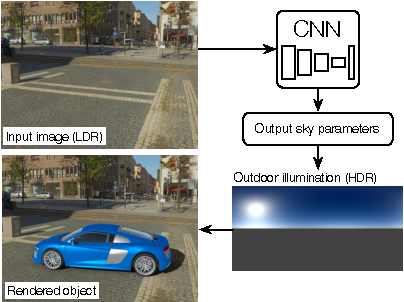
\includegraphics[width=\linewidth]{figures/teaser/teaser-skymodel.pdf}
\caption{We present an approach for predicting full HDR lighting conditions from a single LDR outdoor image. Our prediction can readily be used to insert a virtual object into the image. Our key idea is to train a CNN using input-output pairs of LDR images and HDR illumination parameters that are automatically extracted from a large database of $360^\circ$ panoramas.}
\label{fig:teaser}
\vspace{-1em}
\end{figure}

Illumination plays a critical role in deciding the appearance of a scene, and recovering scene illumination is important for a number of tasks ranging from scene understanding to reconstruction and editing. However, the process of image formation conflates illumination with scene geometry and material properties in complex ways and inverting this process is an extremely ill-posed problem. This is especially true in outdoor scenes, where we have little to no control over the capture process.

Previous approaches to this problem have relied on extracting cues such as shadows and shading~\cite{lalonde-ijcv-12} and combining them with (reasonably good) estimates of scene geometry to recover illumination. However, both these tasks are challenging and existing attempts often result in poor performance on real-world images. Alternatively, techniques for intrinsic images can estimate low-frequency illumination but rely on hand-tuned priors on geometry and material properties~\cite{barron-pami-15,lombardi2016reflectance} that may not generalize to large-scale scenes. In this work, we seek a single image outdoor illumination inference technique that generalizes to a wide range of scenes and does not make strong assumptions about scene properties.

To this end, our goal is to train a CNN to directly regress a single input low dynamic range image to its corresponding high dynamic range (HDR) outdoor lighting conditions. Given the success of deep networks at related tasks like intrinsic images~\cite{zhou2015intrinsic} and reflectance map estimation~\cite{rematas-cvpr-16}, our hope is that an appropriately designed CNN can learn this relationship. However, training such a CNN requires a very large dataset of outdoor images with their corresponding HDR lighting conditions. Unfortunately, such a dataset currently does not exist, and, because capturing light probes requires significant time and effort, acquiring it is prohibitive.

Our insight is to exploit a large dataset of outdoor panoramas~\cite{xiao-cvpr-12}, and extract photos with limited field of view from them. We can thus use pairs of photos and panoramas to train the neural network. However, this approach is bound to fail since: 1) the panoramas have low dynamic range and therefore do not provide an accurate estimate of outdoor lighting; and 2) even if notable attempts have been made~\cite{zhang-cvpr-13}, recovering full spherical panoramas from a single photo is both improbable and unnecessary for a number of tasks (e.g., many of the high-frequency details in the panoramas are not required when rendering Lambertian objects into the scene).

Instead, we use a physically-based sky model---the Ho\v{s}ek-Wilkie model~\cite{hosek-siggraph-12,hosek-cga-13}---and fit its parameters to the visible sky regions in the input panorama. This has two advantages: first, it allows us to recover physically accurate, high dynamic range information from the panoramas (even in saturated regions). Second, it compresses the panorama to a compact set of physically meaningful and representative parameters that can be efficiently learned by a CNN. At test time, we recover these parameters---including sun position, atmospheric turbidity, and geometric and radiometric camera calibration---from an input image and use them to construct an HDR sky environment map. 

To our knowledge, we are the first to address the complete scope of estimating a full HDR lighting representation---which can readily be used for image-based lighting~\cite{Debevec1998}---from a single outdoor image (fig.~\ref{fig:teaser}). Previous techniques have typically addressed only aspects of this problem, e.g., Lalonde et al.~\cite{lalonde-ijcv-12} recover the position of the sun but need to observe sky pixels in order to recover the atmospheric conditions. Similarly,~\cite{Ma2017} uses a neural network to estimate the sun azimuth to perform localization in roadside environments. Karsch et al.~\cite{karsch2014automatic} estimate full environment map lighting, but their panorama transfer technique may yield illumination conditions arbitrarily far away from the real ones. In contrast, our technique can recover an accurate, full HDR sky environment map from an arbitrary input image. We show through extensive evaluation that our estimates of the lighting conditions are significantly better than previous techniques and that they can be used ``as is'' to photorealistically relight and render 3D models into images.    



